%% Template.tex; Solar Physics
%% 
\documentclass[namedreferences]{solarphysics}
%
% spr-sola-addons available options:
%  natbib        -- For citations: redefine \cite commands (loads natbib.sty)
%  solaenum      -- makes enumerated list with italics-roman numerals and a single right-bracket
%  solaromanenum -- makes enumerated list with roman numerals and a single right-bracket
%  linksfromyear -- puts a link on a year citation (hyperref must be loaded)
%  optionalrh    -- for optional running title/author
%
\usepackage[optionalrh,solaromanenum]{spr-sola-addons} % For Solar Physics 
%\usepackage{epsfig}                     % For eps figures, old commands
\usepackage{graphicx}                    % For eps figures, newer & more powerfull
%\usepackage{courier}                    % Change the \texttt command to courier style
%\usepackage{amssymb}                    % useful mathematical symbols
\usepackage{color}                       % For color text: \color command
\usepackage{url}                         % For breaking URLs easily trough lines
\def\UrlFont{\sf}                        % define the fonts for the URLs


%% Local definitions
%% please place your own definitions here and don't use \def but
%% \newcommand{}{} or 
%% \renewcommand{}{} if it is already defined in LaTeX
\newcommand{\solphys}{{\it Solar Physics}}
\newcommand{\aap}{    {\it Astronomy \& Astrophysics}}
\newcommand{\aaps}{   {\it Astronomy \& Astrophysics Supplemental}}
\newcommand{\apj}{    {\it Astrophysical Journal}}
\newcommand{\apjl}{    {\it Astrophysical Journal Letters}}
\newcommand{\apjs}{	{\it Astrophysical Journal Supplement}}
\newcommand{\jgr}{    {\it Journal of Geophysical Research}}
\newcommand{\aapr}{    {\it Astronomy \& Astrophysics Review}}
\newcommand{\grl}{    {\it Geophysical Research Letters}}
\newcommand{\lrsp}{    {\it Living Rev. Solar Phys.}}



%%%%%%%%%%%%%%%%%%%%%%%%%%%%%%%%%%%%%%%%%%%%%%%%%%%%%%%%%%%%%%%%%%
\begin{document}

\begin{article}

\begin{opening}

\title{Bridging EUV and white-light observations using the \emph{PROBA2}/SWAP imager and MLSO/MK4 coronagraph: evidence for the breakout model in a ``two-stage" solar eruptive event.}

%%%%%%%%%%%%%%%%%%%%%%%%%%%%%%%%%%%%%%%%%%%%%%%%%%%
%% Authors Names
%
\author{J.\,P.~\surname{Byrne}$^{1}$\sep
        et al.
%	H.~\surname{Morgan}$^{3,1,4}$\sep
%	D.\,B.~\surname{Seaton}$^{2}$\sep
%	S.\,R.~\surname{Habbal}$^{1}$ 
%	H.\,M.~\surname{Bain}$^{5}$     
       }

%%%%%%%%%%%%%%%%%%%%%%%%%%%%%%%%%%%%%%%%%%%%%%%%%%%
%% Runningheads
%
\runningauthor{Byrne et al.}
\runningtitle{SWAP}


%%%%%%%%%%%%%%%%%%%%%%%%%%%%%%%%%%%%%%%%%%%%%%%%%%%
%% Affilations 
%
  \institute{$^{1}$Institute for Astronomy, University of Hawai'i, 2680 Woodlawn Drive, Honolulu, HI 96822, USA.
                     email: \url{jbyrne@ifa.hawaii.edu} %email: \url{e.mail-b}%\\ 
%	$^{2}$Royal Observatory of Belgium, Avenue Circulaire 3, 1180 Brussels, Belgium.
%	$^{3}$Sefydliad Mathemateg a Ffiseg, Prifysgol Aberystwyth, Ceredigion, Cymru, SY23 3BZ, UK.
%	$^{4}$Coleg Cymraeg Cenedlaethol, Y Llwyfan, Ffordd y Coleg, Caerfyrddin, Cymru, SA31 3EQ, UK.
%	$^{5}$Space Sciences Laboratory, University of California, Berkeley, CA 94720-7450, USA.
%                     email: \url{e.mail-c} \\
             }


%%%%%%%%%%%%%%%%%%%%%%%%%%%%%%%%%%%%%%%%%%%%%%%%%%%
%%% Abstract 
\begin{abstract}
The initiation phase of CMEs is a very important aspect of solar physics, being an indication of the magnetic reconnection process that must be occurring to facilitate the shedding of helicity in the solar cycle. The interesting physics at play is known to occur between the photosphere and low corona, where many models introduce an instability that triggers a CME; be it due to internal or external tether-cutting processes or other such changes to the magnetic field topology that may drive an eruptive event, often with associated flaring activity. To this end, it is worthwhile to obtain a variety of observations of the low corona, with different passbands, cadences, and fields--of-view, in order to build as clear a picture as possible of the dynamics that occur therein. Here, we combine the EUV imagery of the SWAP instrument onboard \emph{PROBA2} with the white-light imagery of the ground-based MK4 coronagraph in order to bridge the observational gap that exists between the disk imagery of AIA onboard \emph{SDO} and the coronal imagery of LASCO onboard \emph{SOHO}. Methods of multiscale image analysis were applied to the SWAP and MK4 observations to reveal CME structure while suppressing noise and other features. This allowed an investigation into the initiation phase of a CME of particular interest due predominantly to the ``two-stage" flaring profile of its associated active region that underlay an extended helmet streamer. Previous evidence for interchange reconnection in the helmet streamer was observed, along with a dramatic restructuring of the magnetic field via an M-class flare prior to the CME flux rope formation and eruption. Once formed, it was found that the outward motion of the flux rope in the EUV observations lagged behind the bulk motion of the white-light CME core material, while the overall system expanded into the helmet streamer to become the larger CME structure observed in the coronagraph images. Furthermore, the characterised CME core (attributed to the flux rope) was determined to undergo a strong jerk in its motion, as the early acceleration jumped abruptly from $\sim$20$\,m\,s^{-2}$ to $\sim$130$\,m\,s^{-2}$ in line with the second-stage flaring and overall CME eruption through the LASCO field-of-view, which later became concave-outward in shape. These observations provide evidence for the breakout model, specifically in the case of a streamer blowout. 



 %The methods use successive filtering of an image via a Gaussian and derivative-of-Gaussian produces a number of scales of detail to be inspected. This also produces an image with intensities that represent the relative edge strengths in the original image, which can be used to characterize the structure of interest -- specifically for this case the erupting material involved in the CME. In order to overlap the observations from SWAP and MK4, the core material of the CME in its early eruption phase was chosen for its higher signal to noise ratio than the CME front, for example, that was not discernible in the early stages of the observations. In the LASCO field-of-view, the core material was determined to be moving at the same speed as the CME front, at $\sim$\,500$\,km\,s^{-1}$. The front portion of the core material in the MK4 images was characterized via point-\&-click methodology on the multiscale images of enhanced edges, and an ellipse was fit to the curved front. The same was done for the erupting loop structure observed in SWAP, with the expectation that it might directly correlate to the CME core. However, it was found that the erupting material that starts at the same time and location in both the MK4 and SWAP images, did not proceed to erupt at the same rate. Rather the core material observed in MK4 moves at greater speeds than the loop structures observed in SWAP; rising from an initial speed of $\sim$\,100$\,km\,s^{-1}$ (at $\sim$\,1.5$\,R_{\odot}$) to a final speed of $\sim$\,400$\,km\,s^{-1}$ (at $\sim$\,2$\,R_{\odot}$), while the loops continue to steadily rise at $\sim$\,100$\,km\,s^{-1}$. The reason for this is unclear, and requires further investigation.
 
\end{abstract}



%%%%%%%%%%%%%%%%%%%%%%%%%%%%%%%%%%%%%%%%%%%%%%%%%%%
%% Keywords
%
\keywords{Coronal Mass Ejections, Low Coronal Signatures, Initiation and Propagation}


\end{opening}
%-------------------------------------------------

%%%%%%%%%%%%%%%%%%%%%%%%%%%%%%%%%%%%%%%%%%%%%%%%%%%
%% Sections
%

\section{Introduction}
\label{intro}

Coronal mass ejections (CMEs) represent the largest, most dynamic phenomena that originate from the Sun. Propagating at speeds of hundreds up to thousands of kilometers per second \cite{2004JGRA..10907105Y}, the particle densities and energies involved can cause adverse space weather at Earth and elsewhere in the heliosphere \cite{2005AnGeo..23.1033S}. They can lead to geomagnetic storms upon impacting our magnetosphere, damaging satellites, affecting communication and navigation systems, and increasing the radiation risk for astronauts \cite{2007A&G....48f..11L}. Given their potentially hazardous impact on Earth�s geomagnetic environment, the physics governing their eruption and propagation needs to be understood. 

Various theoretical CME models exist in the effort to reproduce the physical driver mechanisms responsible for their initiation and propagation (see the review by \opencite{2011LRSP....8....1C}). All are based upon the requirement that some form of instability must trigger the eruption, most likely as a result of a magnetic energy imbalance often described in the context of tether straining and release \cite{2001AGUGM.125..143K}. Considering the underlying structure of the CME as a flux rope (e.g., \opencite{1996JGR...10127499C}), possible causes for eruption may include flux injection and magnetic twisting \cite{2006PhRvL..96y5002K,2001ApJ...562.1045K}, reconnection beneath the flux rope \cite{2007ApJ...658L.123L,2003ApJ...595.1231A}, or breakout reconnection between the overlying field and neighboring flux systems \cite{2008ApJ...683.1192L,2007ApJ...671L..77V}. Such models may provide an interpretation on observations, and thus allow some deeper understanding of the forces governing CMEs and their relationship with associated phenomena like flares.

%Several theoretical models are described by \cite{Krall01} within the context of the magnetic flux rope model of \cite{Chen96}. These include flux injection, magnetic twisting, magnetic energy release and hot plasma injection. The three-dimensional magnetic flux rope model, in which a converging flow toward the neutral line results in reconnection beneath the flux rope \cite{Forbes95, Amari03, Lin07}, assumes that the kinematics of an erupting flux rope can be described using a force-balance equation, which includes gas pressure, gravity and the Lorentz force \cite{KrallChen05, Chen06, Manchester07}. An alternative to this is the magnetic break-out model in which the CME eruption is triggered by reconnection between the overlying field and a neighbouring flux system \cite{Antiochos99, Lynch04, MacNeice04}. The increased rate of outward expansion drives a faster rate of breakout reconnection yielding the positive feedback required for an explosive eruption. The models are dependent on geometrical properties of the CME, such as its width and radius, and they are designed to give an indication of the processes that drive CME kinematics. Thus it is important to develop methods of localising the CME front and characterising it in the observed data with high accuracy for model comparisons.


An important aspect of studying CME initiation, is the ability to resolve their low-corona propagation and associated source regions on the disk: be it a flaring or non-flaring active region, a prominence/filament eruption or other rising loop system \cite{2002ApJ...566L.117Z,2001ApJ...561..372S}, or else a ``stealth CME" without any specifically detectable source \cite{2013SoPh..285..269H}. Prominence lift-offs often become the core material of a CME \cite{2008AnGeo..26.3025F,2003ApJ...586..562G}, and rising loops often form some part of the CME morphology \cite{2006A&A...455..339D,2004A&A...422..307C}. Their low-corona kinematics and morphology provide insight into the early forces at play, and so a rigorous study of such phenomena is key to understanding the physics involved.

\begin{figure}[ht]
\centering{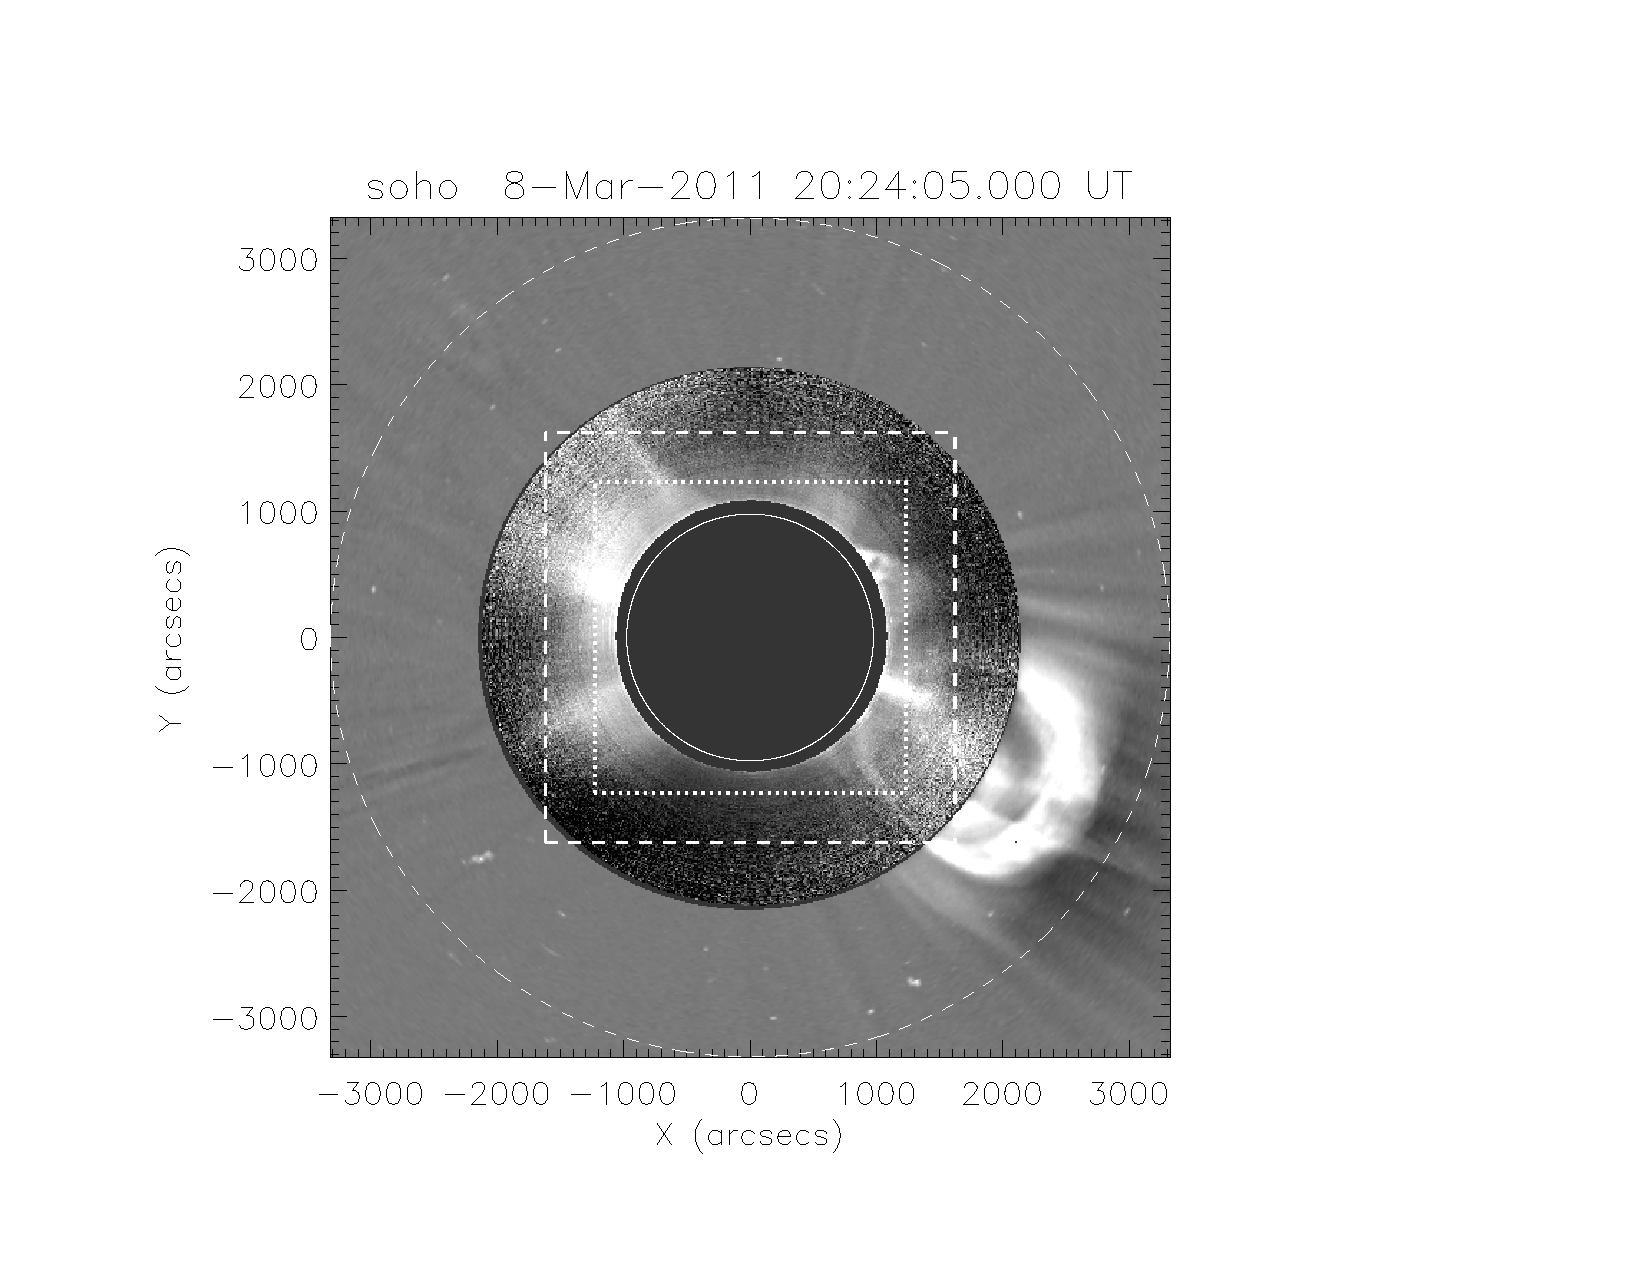
\includegraphics[scale=0.43, trim=60 50 200 70]{images/overlays.pdf}}
\caption{A LASCO/C2 image with an MLSO/MK4 image overlaid in the range 1.1\,--\,2.2\,$R_\odot$, dated 8~March~2011 at 20:24 and 20:22~UT respectively. The C2 image has been processed via the CORIMP techniques of normalizing radial graded filter (NRGF) and quiescent background subtraction. It has been trimmed to a half-width of 3.4\,$R_\odot$, which is the upper limit of the \emph{PROBA2}/SWAP field-of-view as indicated by the dashed circle. The SWAP field-of-view during nominal operations is indicated by the dashed box. The \emph{SDO}/AIA field-of-view is indicated by the inner dotted box. The limb of the Sun behind the occulter is indicated by the solid white circle. A CME is observed off the south-west limb as a bright loop structure with some inner core material, as seen here in the Thomson-scattered white-light coronagraph images. It is clear how the SWAP and AIA images can be used to bridge CME observations to the low corona and solar disk, for gaining insight to their initiation phase.}
\label{overlays}
\end{figure}

In order to connect CMEs to their source regions, data from disk imagers such as the Sun Watcher using APS detectors and image Processing (SWAP; \opencite{2013SoPh..286...43S}) onboard the second Projects for Onboard Autonomy (\emph{PROBA2}; \opencite{2013SoPh..286....5S}) and the Atmospheric Imaging Assembly (AIA; \opencite{2012SoPh..275...17L}) onboard the Solar Dynamics Observatory (\emph{SDO}; \opencite{2012SoPh..275....3P}), may be used in tandem with coronagraph observations. However, difficulties in the interpretation of the observed features arise due to the varying instrument specifications, e.g., image passbands, fields-of-view, cadences, etc. Therefore, to bridge the gap between the white-light images of the extended corona and the EUV observations of the solar disk and low corona, the SWAP imager was used in conjunction with the Mauna Loa Solar Observatory (MLSO) MK4 coronagraph \cite{2003SPIE.4843...66E} to directly compare the observations of CMEs as they erupt through the overlapping fields-of-view (Fig.\,\ref{overlays}). This allows a direct correspondence of features in the EUV images with those in the white-light images, providing new insight into the connection of CMEs to the Sun during their initial phases of eruption and acceleration away from their source regions on the disk.

A difficulty exists in studies of coronal structure that are prone to low signal-to-noise ratios in the observational data. Low-coronal white-light observations using a coronagraph are problematic due to the strong radial brightness gradient and issues with scattered light in the instrument, while extended EUV disk observations are problematic due to the strong drop-off in emission brightness with increasing coronal height. These common issues with solar observational data motivate the development and use of advanced image processing techniques to suppress noise and enhance structures in the image data \cite{2011ApJ...737...88D,2011AdSpR..47.2118G,2011igi-global,2008ApJ...674.1201S,2008SoPh..248..457Y,2006SoPh..236..263M,2003A&A...398.1185S}. 

In Section\,\ref{sect:techniques} we describe the use of multiscale image processing methods on SWAP and MK4 data. In Section\,\ref{sect:event} we present a case-study of a flux rope that erupted on 8~March~2011, to provide deeper insight to the initiation phase of CMEs. A discussion of the interpretation of this study is presented in Section\,\ref{sect:discussion}.

\section{Observations \& Techniques}
\label{sect:techniques}

\begin{figure}[t]
\centering{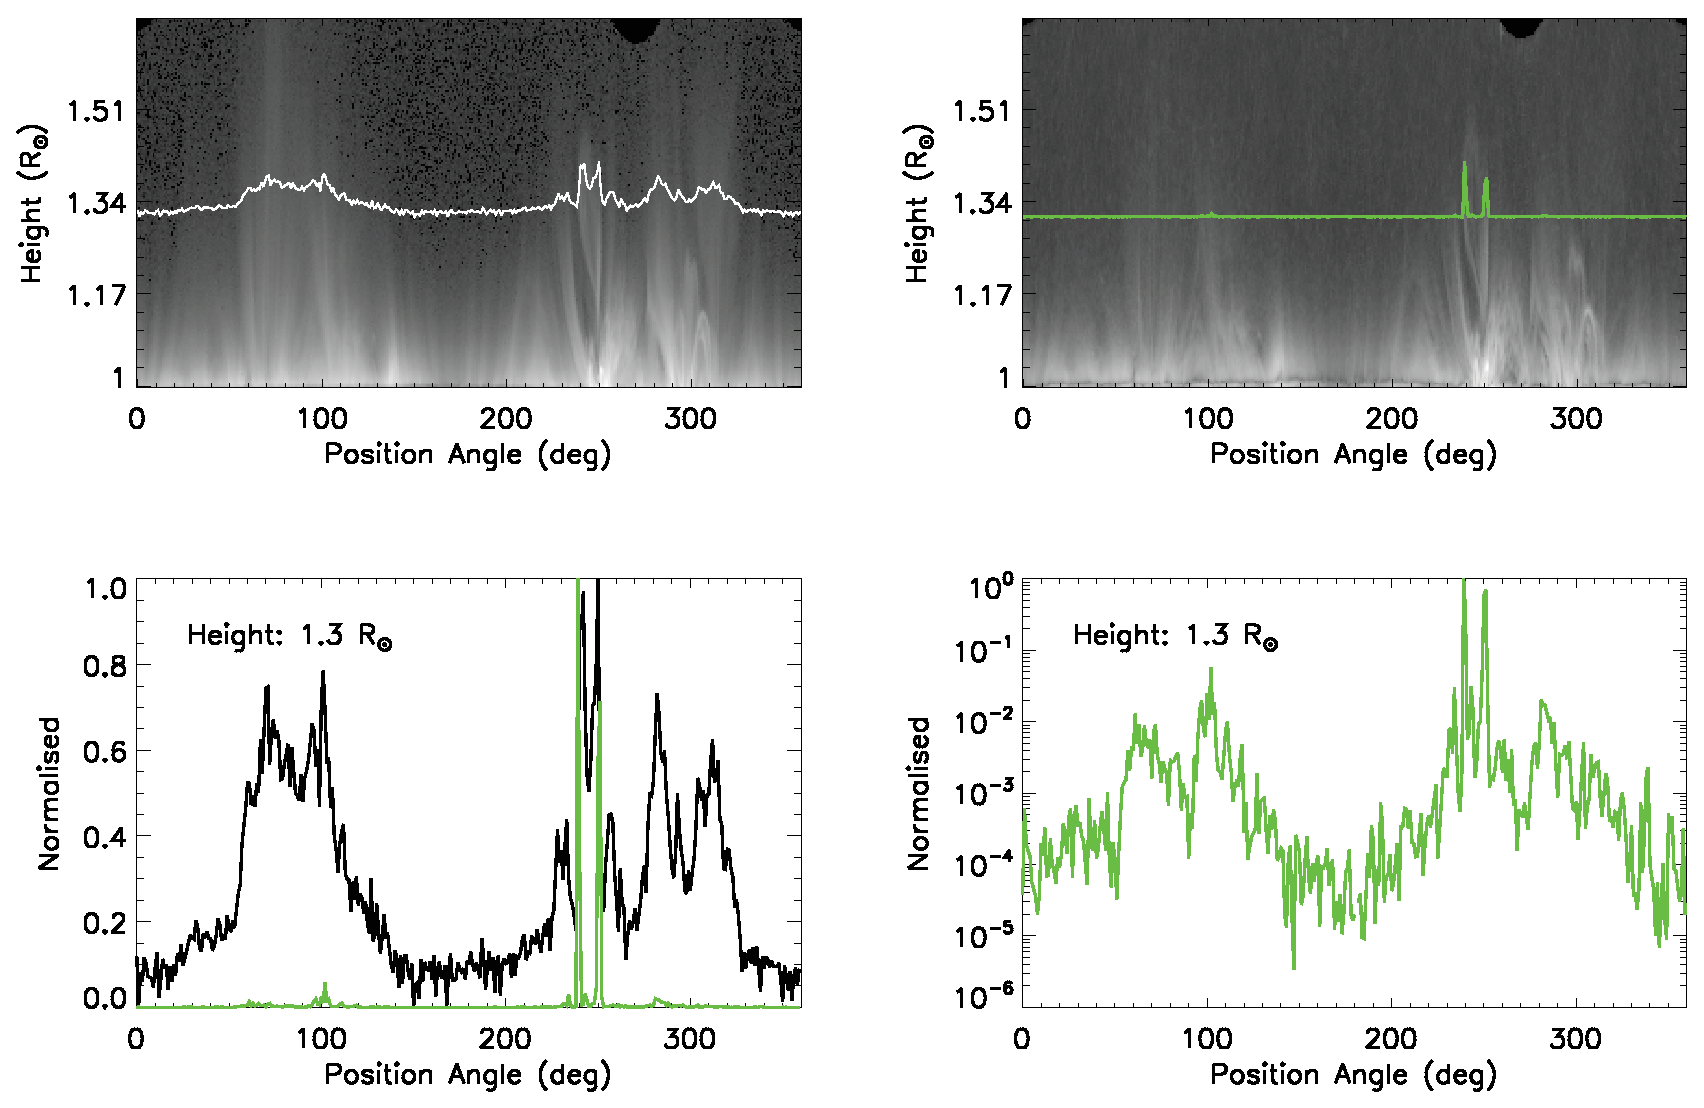
\includegraphics[scale=0.425, trim=25 0 15 0, clip=true]{images/polar_fig_swap_20110308.eps}}
\caption{The top two panels show polar-unwrapped images of the solar corona across the \emph{PROBA2}/SWAP field-of-view on 8~March~2011 at 19:53:59\,UT; left being the level-1 data, right being the enhanced data. Across each image, at a constant height of 1.3~R$_\odot$, an intensity slice is plotted (of arbitrary normalised units) to demonstrate how the background coronal structure is suppressed by the multiscale techniques, to highlight only the complex structure of the prominence. The bottom left plot shows a direct comparison of the two intensity slices, where the prominence is located between 230\,--\,260$^\circ$. The bottom right plot shows a log scale of the normalised intensity slice across the enhanced image to demonstrate that the rest of the coronal structure is still present, just strongly suppressed relative to the prominence material.}
\label{polar_fig_swap_20110308}
\end{figure}


Methods of multiscale image processing have been developed in recent years for use on coronagraph images to enhance the underlying structure. The fundamental idea behind these methods is to highlight details apparent on different scales within the data. Therefore, multiscale techniques provide an ability to remove small-scale features in images, essentially suppressing the noise such that the structures of interest can be revealed in greater detail. By applying them to coronagraph images, the morphology of CMEs as they propagate through the corona in a sequence of observations can be determined with better accuracy than previously possible (\opencite{2009A&A...495..325B}, \citeyear{2012ApJ...752..145B}). 

These methods are now demonstrated for use on the MK4 coronagraph and SWAP EUV imager, to provide insight to the low-coronal morphology of erupting structures that may form CMEs. Details on the fundamental technique are outlined in \inlinecite{2008SoPh..248..457Y} wherein the magnitude of the multiscale gradient is used to show the relative strength of the detected edges in the image structure at a particular scale of the multiscale decomposition (i.e., the strongest edges appear brightest). To increase the signal-to-noise ratio of the edge detections further, the magnitude information from the scales most relevant to the coronal structures of interest may be multiplied together, neglecting the largest scales that smooth out the coronal signal, and the smallest scales that reveal the finer structure and noise (see \opencite{2012ApJ...752..145B}, for details). Thus the magnitude of the multiscale gradient across the dominant edges of coronal loops and CMEs is further enhanced for subsequent characterization of their morphology. 

Figure\,\ref{polar_fig_swap_20110308} shows the effectiveness of the multiscale techniques for detecting the structure of an ejection observed by SWAP at 19:53:59\,UT on 8~March~2011. The top left image shows the level-1 processed data, polar-unwrapped about Sun-center at coronal heights of 1--1.7\,R$_{\odot}$. The top right image shows the result of the multiscale filtering technique applied in such a manner as to enhance the edges of the detected structure in the data. The bottom left plot shows the comparison of an intensity slice at a height of 1.3\,R$_{\odot}$ in each, revealing how the multiscale techniques best characterize the complex structure of the erupting prominence material. The bottom right plot then shows a log of the intensity slice across the multiscale filtered image to reveal the suppressed signal of the background features.


\begin{figure}[t]
\centering{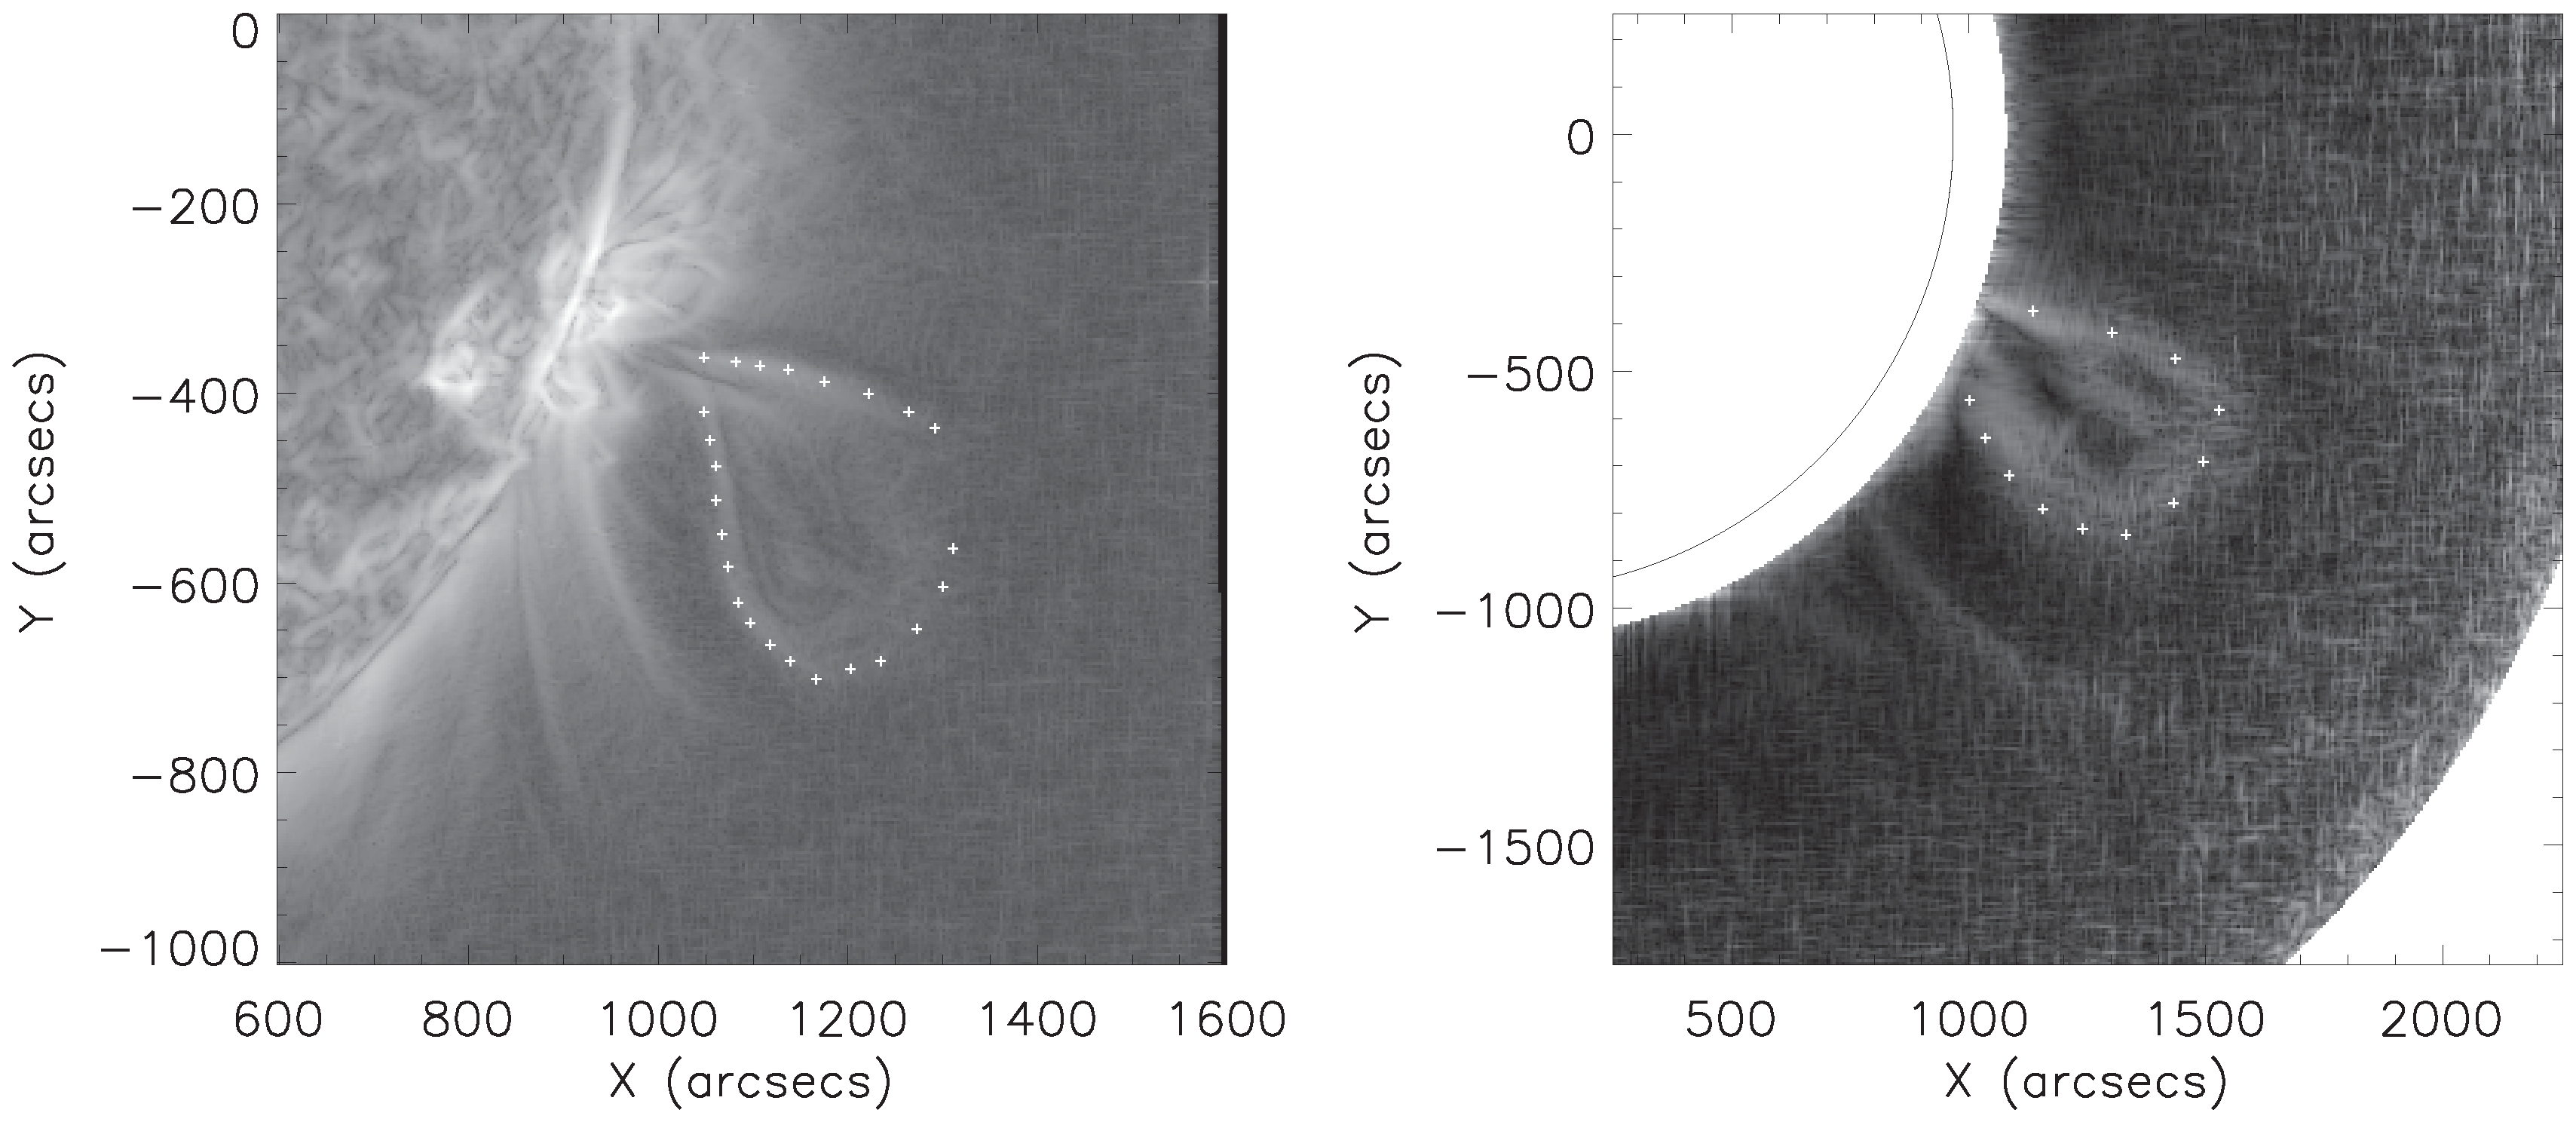
\includegraphics[scale=0.2, trim=0 40 0 0, clip=true]{images/combined_modgrad_points.eps}}
\caption{SWAP (left) and MK4 (right) observations of the erupting loop system that forms the inner core of the CME on 8~March~2011, at times 19:53:59 and 19:56:16\,UT respectively. The images have been processed via the multiscale decomposition, showing here intensities that represent the magnitude of the detected edges.}
\label{combined_modgrad_points}
\end{figure}


The extended corona from $\sim$\,2\,--\,30\,$R_{\odot}$ is often observed with the Large Angle Spectrometric Coronagraph (LASCO; \opencite{1995SoPh..162..357B})  onboard the Solar and Heliospheric Observatory (SOHO; \opencite{1995SoPh..162....1D}) situated about the L1 point. (Along with the more recently launched SECCHI coronagraphs onboard the STEREO mission, from increasing angles of separation in their orbits about the Sun.) Coronal structures, and specifically CMEs, have been studied in the white-light image data from these instruments through the use of a number of steps outlined in the Coronal Image Processing package (CORIMP; \opencite{2012ApJ...752..144M}, \opencite{2012ApJ...752..145B}). These techniques have now been extended for use on the MLSO/MK4 coronagraph data, which provides white-light polarization brightness images of the corona from $\sim$\,1.14\,--\,2.86\,$R_{\odot}$ at a cadence of approximately 3~minutes. The MK4 data is prepared via an instrumental vignetting function that maximizes the image contrast by offsetting the radial brightness gradient in order to best reveal structures such as CMEs and streamers. A multiscale decomposition is then performed, in order to produce magnitude images of the relative edge strengths in the image to highlight the detected structure (see Fig.\,\ref{combined_modgrad_points}). This allows, for example, an ellipse-fit characterization of the outward propagating fronts, as described in \inlinecite{2009A&A...495..325B}.



\section{``Two-Stage" Eruption of the 8~March~2011 CME}
\label{sect:event}

A CME erupted from the southwest active region NOAA\,11165 at approximately 19:30\,UT on 8~March~2011. The active region caused numerous flares during its evolution across the disk, notably an M4.4 flare at GOES start-time 18:08\,UT (peaking at 18:28\,UT) associated with the rising loop system that later erupted to form the core material of the CME. Of particular interest about this event, is the ``two-stage" X-ray flare profile seen in the GOES flux, identified as two individual M-class flares separated by almost 2 hours. \inlinecite{2012ApJ...746L...5S} present this as clear evidence for a secondary heating phase. The loop system evolution is clearly visible up to $\sim$\,1.3\,$R_{\odot}$ in AIA images, at which height a set of loops that are most strongly observed in AIA-171{\AA} images begin to erupt, being observable to a height of $\sim$\,1.6\,$R_{\odot}$ in the larger field-of-view of the SWAP-174{\AA} imager, and at the time of the secondary M1.4 flare $\sim$\,20:00\,UT. The observations of the active region are exhaustively reported by \inlinecite{2012ApJ...746L...5S}, though it is noted that the system of loops they track (see the stack plot in Fig.\,4 of that paper) is not the same as the flux rope observed and tracked here, which forms at a slightly greater height just off the edge of the AIA field-of-view before the system fully erupts. The CME core is then observed in the white-light MK4 coronagraph images to a height of $\sim$\,2.2\,$R_{\odot}$, entrained within a faint CME bubble that appears to form at these heights before being clearly observed to propagate outwards in the extended LASCO coronagraph images.  %(Fig.\,\ref{lasco_c2_fig}). 

\begin{figure}[t]
\centering{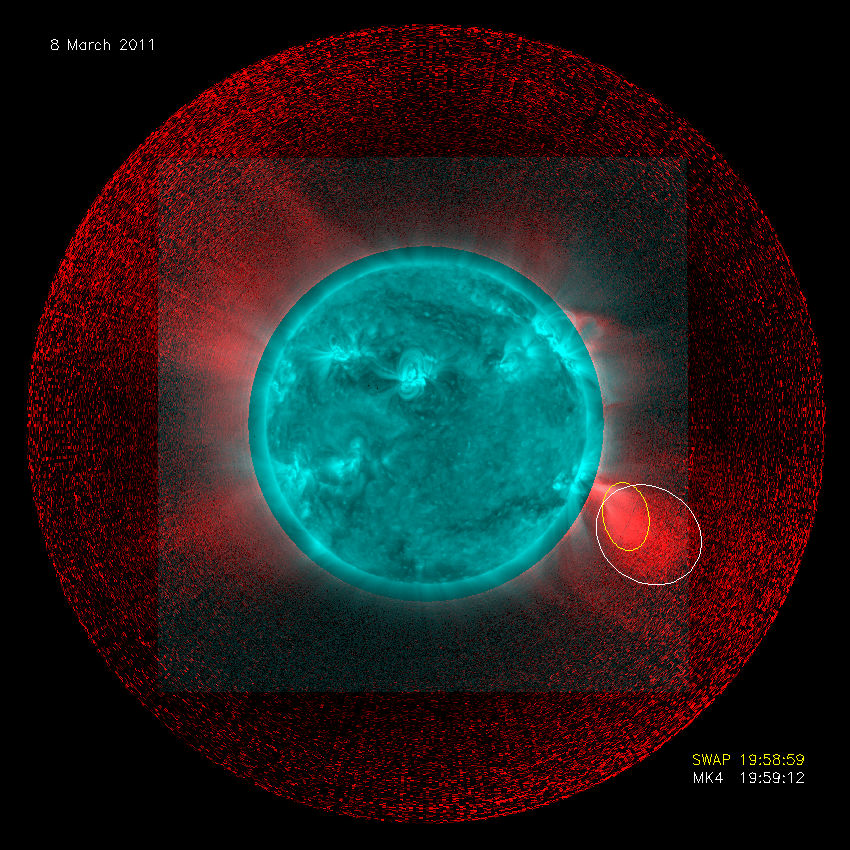
\includegraphics[scale=0.32, clip=true, trim=60 0 0 0]{images/combined.eps}}
\caption{A merged SWAP (blue) and MK4 (red) image with the ellipse-fits to the characterized CME core material as observed by each instrument at 19:59\,UT on 8 March 2011. (An online animation accompanies this figure.)}
\label{combined}
\end{figure}

\inlinecite{2013ApJS..206...19M} report on the expansion of active region loops from this region into the extended solar corona in the day or so leading up to this CME. The region lies beneath a helmet streamer structure that appears to contain the observed coronal loops, with a number of faint brightenings due to small outward-propagating plasma blobs. These, and the pointed shape of the rising loops, are postulated to be indicators of helmet streamer interchange reconnection at the apex of the closed field \cite{2012ApJ...749..182W}. A subsequent brightening and expanding of the loops, accompanied by a swelling of the helmet streamer, precedes the CME from this region and is evidence for an energy input to the system that leads to an explosive energy release. Such a process manifests as the two-stage solar eruptive event outlined in these and \inlinecite{2012ApJ...746L...5S}'s observational studies.

In order to best reveal the eruption material in the low signal-to-noise SWAP and MK4 images, multiscale methods of noise suppression and edge enhancement were employed, as discussed above. This allowed a robust point-\&-click characterization of the CME core material, which was the brightest structure to be tracked through the different imagers when the CME front was not yet fully formed. The rising loop system observed with SWAP and the erupting CME core material observed with MK4 coincided both temporally and spatially with each other, at least initially, and each was characterized by ellipse-fits to the detected front edges of the core flux rope structure. Figure\,\ref{combined} shows an overlay of SWAP and MK4 images during the eruption at times 19:58:59 and 19:59:12\,UT respectively, with the ellipse-fits to the erupting fronts (from point-\&-click characterizations of the edge enhanced multiscale decompositions of the images, as demonstrated in Fig.\,\ref{combined_modgrad_points}). Figure\,\ref{ell_heights_inner} shows the progression of the ellipse-fits to the fronts over the course of the eruption, indicating how the white-light material observed with MK4 propagates away from the source quicker than the EUV material observed with SWAP. The different height-time profiles of the SWAP and MK4 observations are also shown in Fig.\,\ref{ell_heights_inner}, where the material in the MK4 images attains a speed in the range 400\,--\,600\,$km\,s^{-1}$, while the associated erupting loop structures in the SWAP images proceed at only $\sim$\,100$\,km\,s^{-1}$. %The reasons for this are unclear, but the analysis of \inlinecite{2012ApJ...746L...5S} shows that the active region underwent a two-stage flaring process at the time of the eruption that is evidence of a secondary heating phase that coincides with the CME acceleration (Fig.~\ref{kins_CMEcore}). 


\begin{figure}[t]
\centering{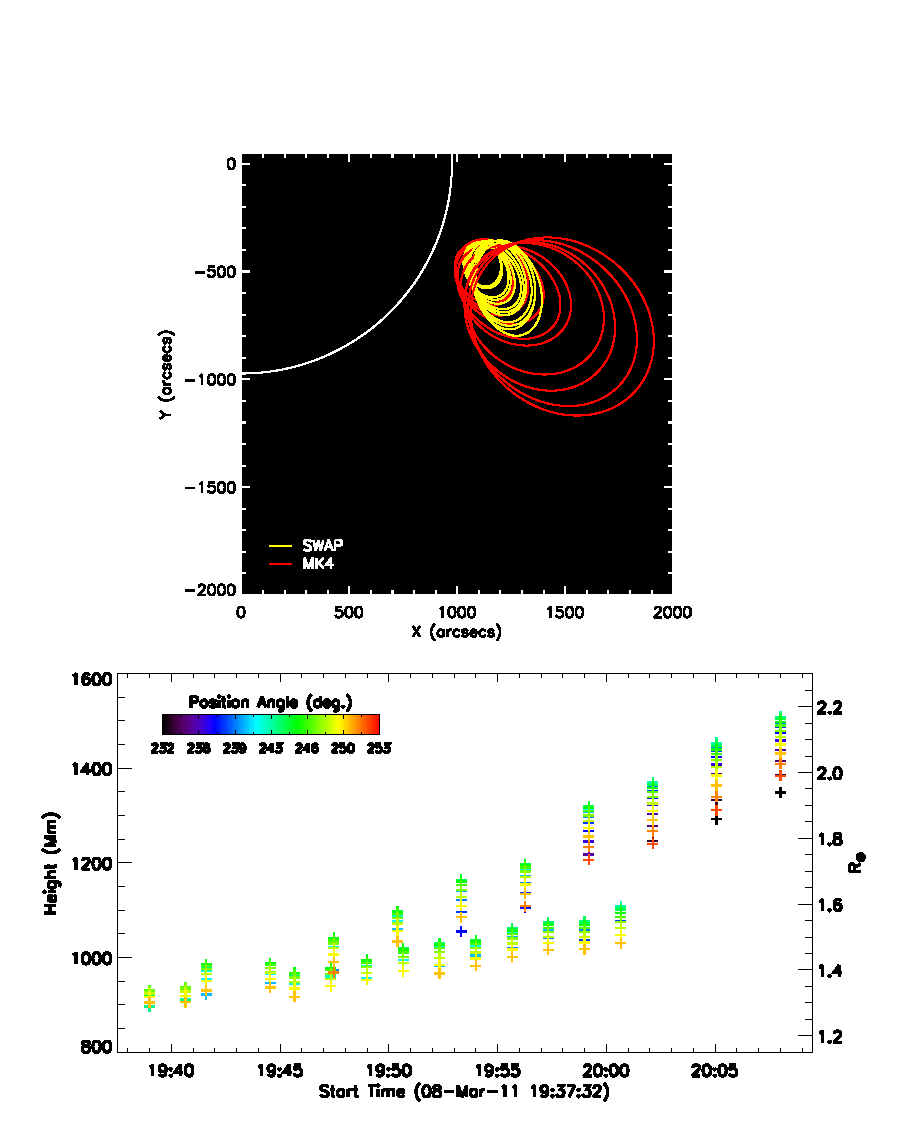
\includegraphics[scale=0.49, clip=true, trim=5 0 10 0]{images/ells_fig.pdf}}
\caption{\emph{Left:} The SWAP and MK4 ellipse-fits to the characterized CME core material over the course of the eruption. \emph{Right:} The height-time profile of the characterized eruption observed simultaneously with the SWAP imager and MK4 coronagraph. The erupting EUV loops move at a speed of $\sim$\,100$\,km\,s^{-1}$ while the associated core of the resulting CME is observed to accelerate up to a speed of $\sim$\,400$\,km\,s^{-1}$.}
\label{ell_heights_inner}
\end{figure}

\begin{figure}[t]
\centering{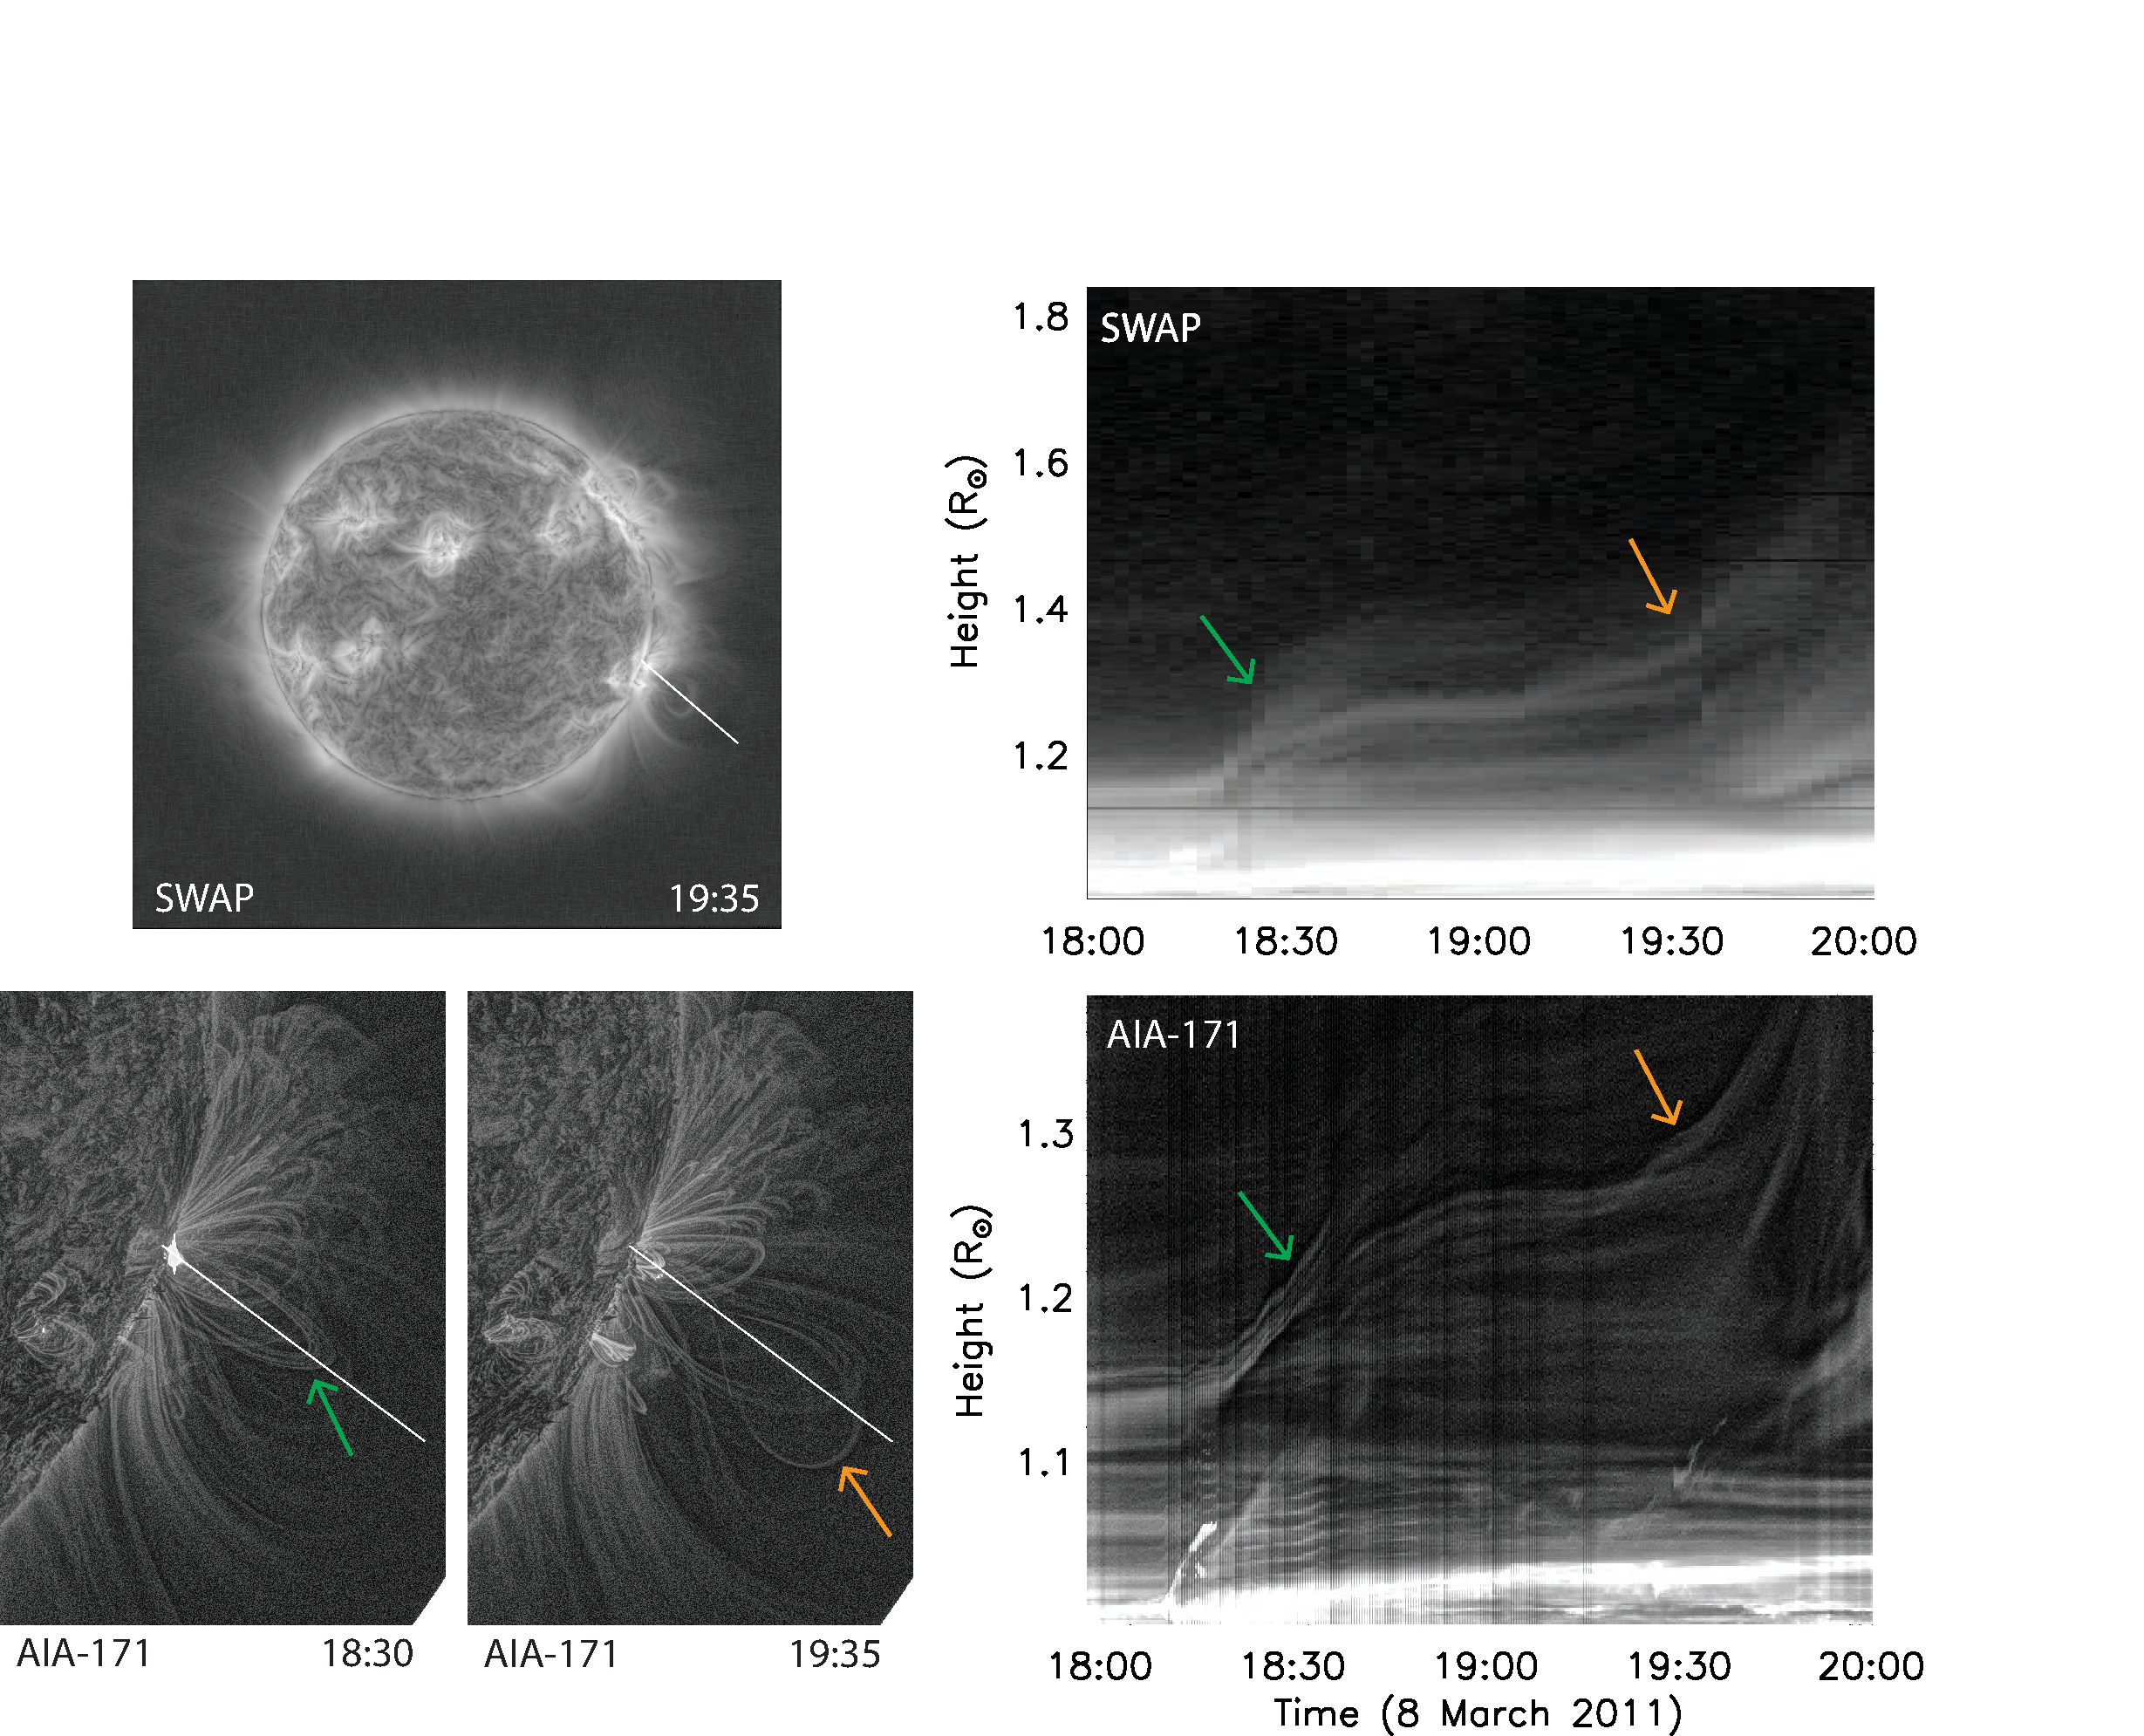
\includegraphics[width=\linewidth, clip=true, trim=0 0 100 150]{images/stackplots.eps}}
\caption{.}
\label{AIA_stackplot_images}
\end{figure}

The CME onset was observed as a series of rising loops, that attained an initial steady height in the low corona of approximately half a solar radii, before destabilizing and becoming the inner core material of a typical three-part CME that propagated out through the corona at a bulk speed of $\sim$\,400$\,km\,s^{-1}$ (based on the kinematics of the CME front detected and tracked in the CORIMP catalog\footnote{http://dublin.ifa.hawaii.edu/$\sim$jbyrne/CORIMP/}). The core of the CME was manually tracked via the multiscale methods and ellipse-fits discussed above (Fig.\,\ref{lasco_c2_fig}), and the resulting kinematics are plotted in Fig.\,\ref{kins_CMEcore}. The height-time measurements of the CME core are shown in color (corresponding to the position angle of the measurements across the plane-of-sky) overlaid on the CME front height-time measurements shown in gray for reference. The Savitzky-Golay filter is used to derive the velocity and acceleration profiles for the CME core; whereby a distribution of velocity and acceleration values is obtained at each data point, with the corresponding median, interquartile range, and upper and lower fences overlaid on each profile as solid, dashed and dotted lines respectively (see \opencite{2013A&A...557A..96B} for a detailed discussion). The inset acceleration phase of the CME core shows initial values of approximately $\sim$\,20$\,m\,s^{-2}$ jumping to $\sim$\,130$\,m\,s^{-2}$ (referred to as the CME jerk by \opencite{2008ApJ...674..586S}). The steepness of this jump may in part be attributed to the numerical effects of the data gap between MK4 and C2, where the spline-fit of the Savitzky-Golay filter (operating on window of 6 neighboring points) compensates somewhat for the jump in velocity that occurs between these two fields-of-view. The magnitude of the velocity, however, was verified by inspection of the different profiles within the separate instrument fields-of-view, for different degrees of polynomial fits and differently sized Savitzky-Golay filters. That is, the rise in velocity is determined to be real, though its true steepness might be better quantified if it were possible to obtain a more complete set of measurements. Nevertheless, it occurs in sync with the second rise in the X-ray flare profile, being an indication of a very fast energy release that allows the explosive eruption of the CME to begin before attaining a speed akin to the local solar wind speed. This double acceleration profile is further evidence of the complexity of this active region whose morphology has been observed to change dramatically over the course of its evolution \cite{2013ApJS..206...19M, 2012ApJ...746L...5S}.

\begin{figure}[t]
\centering{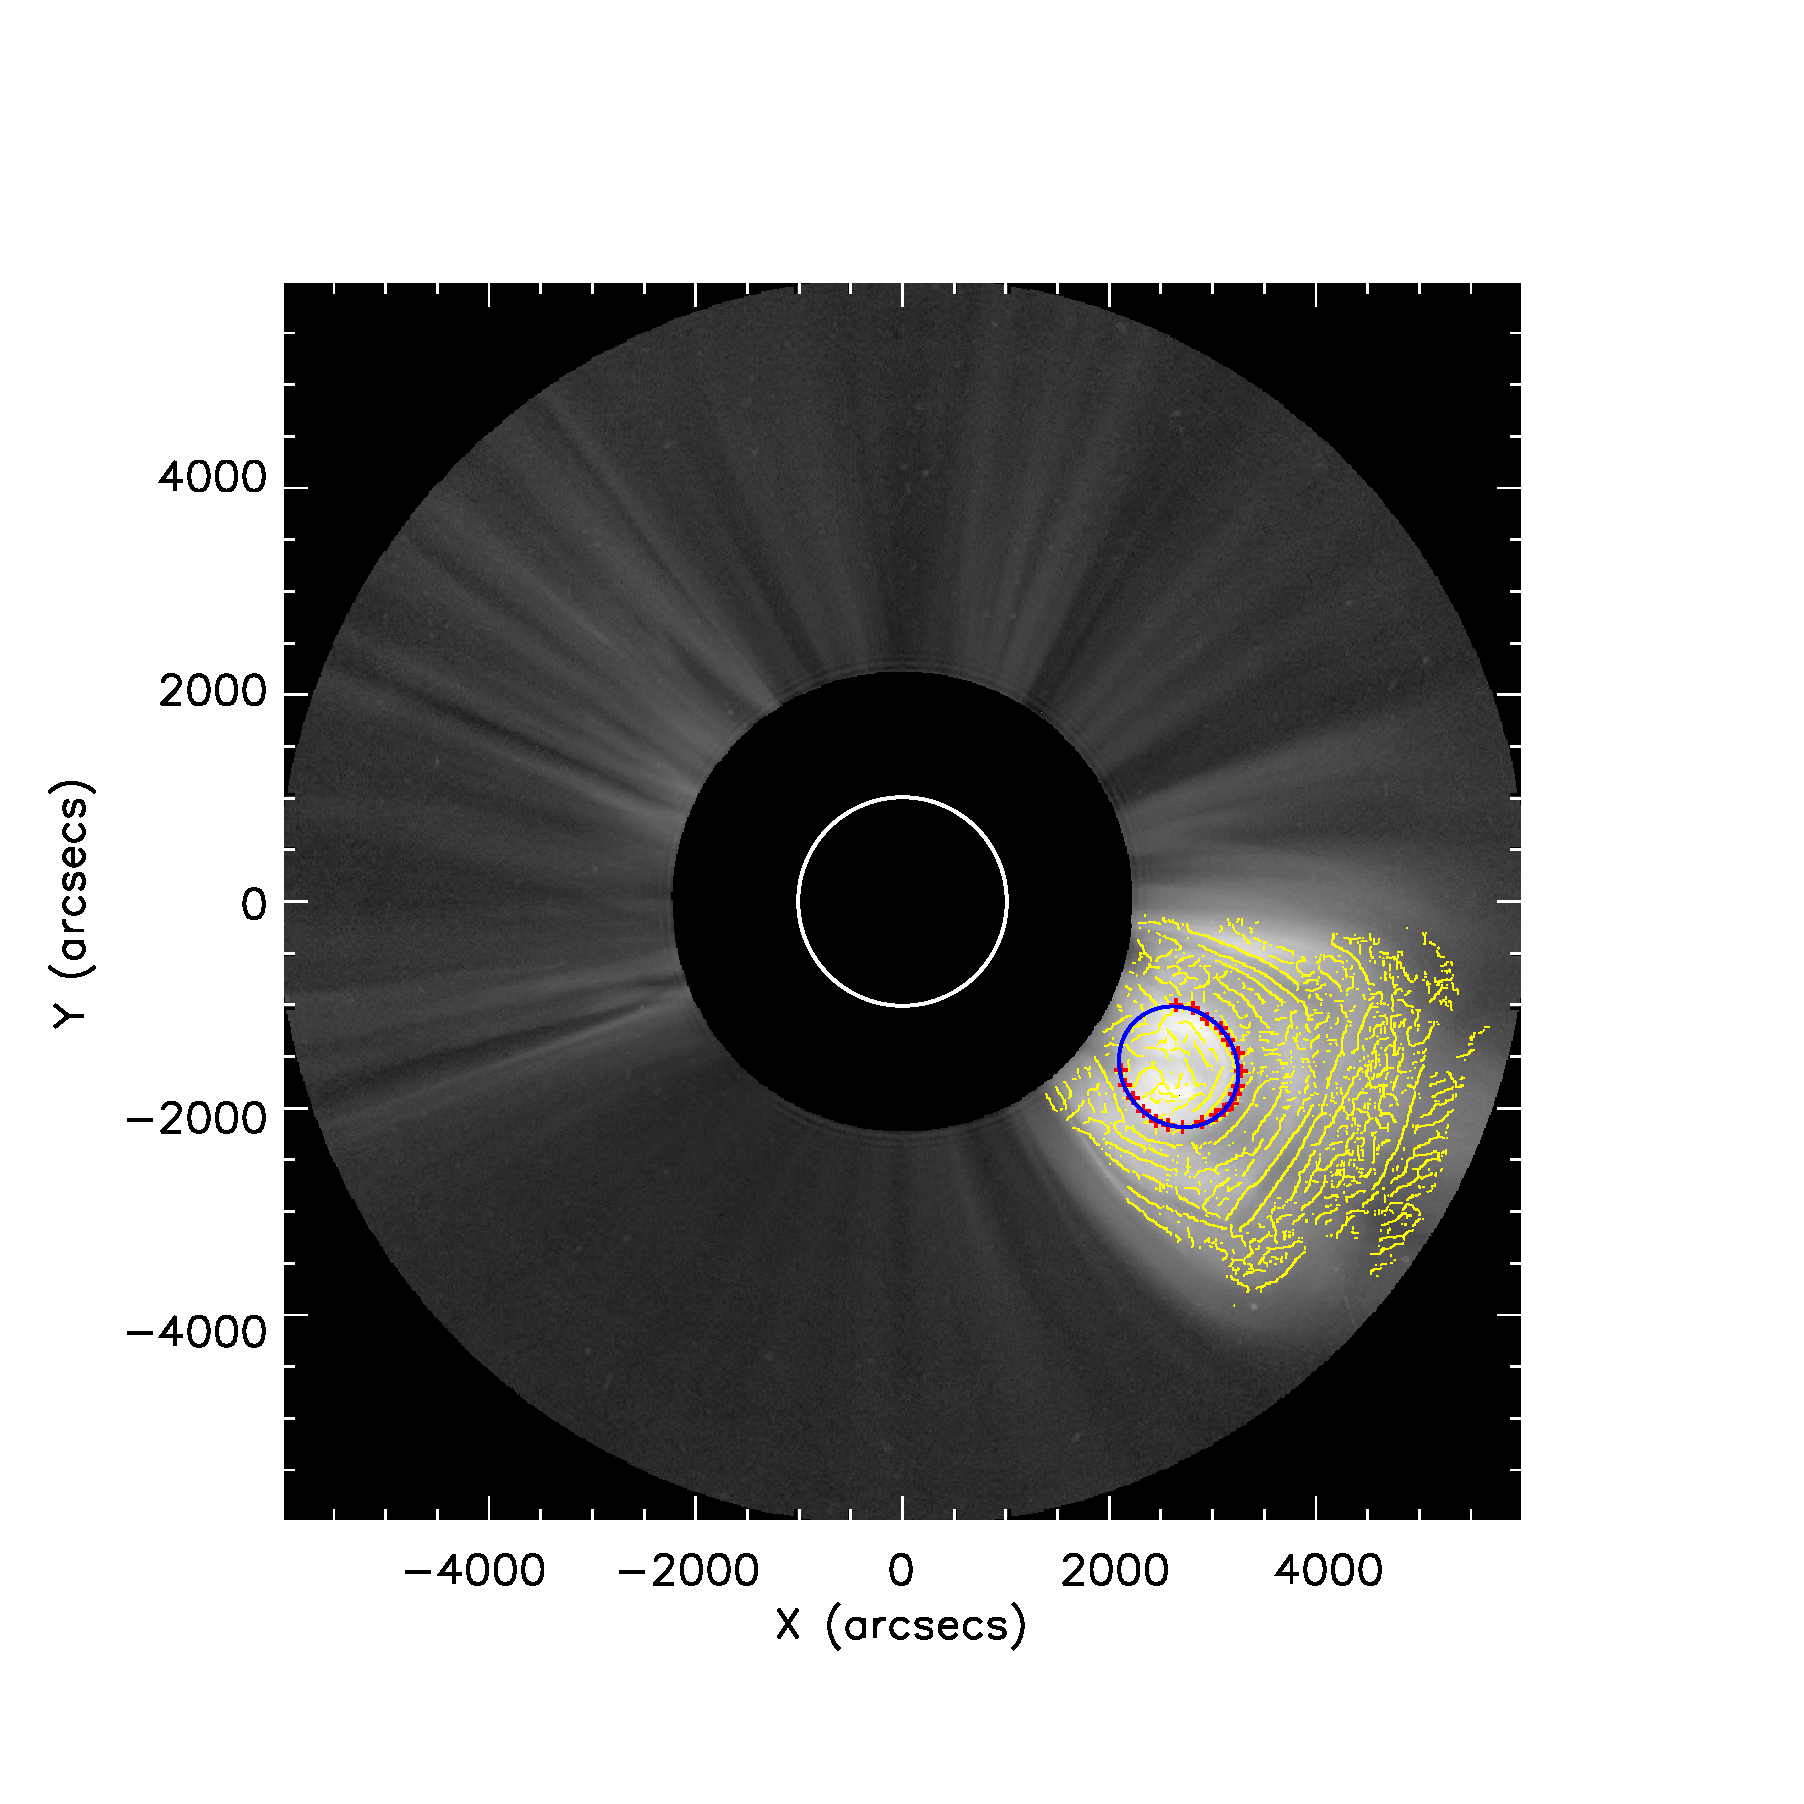
\includegraphics[clip=true, scale=0.27, trim=0 60 0 90]{images/lasco_c2_fig.eps}}
\caption{A radially filtered LASCO/C2 image of the CME at 21:06:51\,UT on 8~March~2011. The yellow contours trace the edges in the detected CME structure, with red points clicked along the corresponding core material, and a resulting ellipse-fit in blue.}
\label{lasco_c2_fig}
\end{figure}

\begin{figure}[!t]
\centering{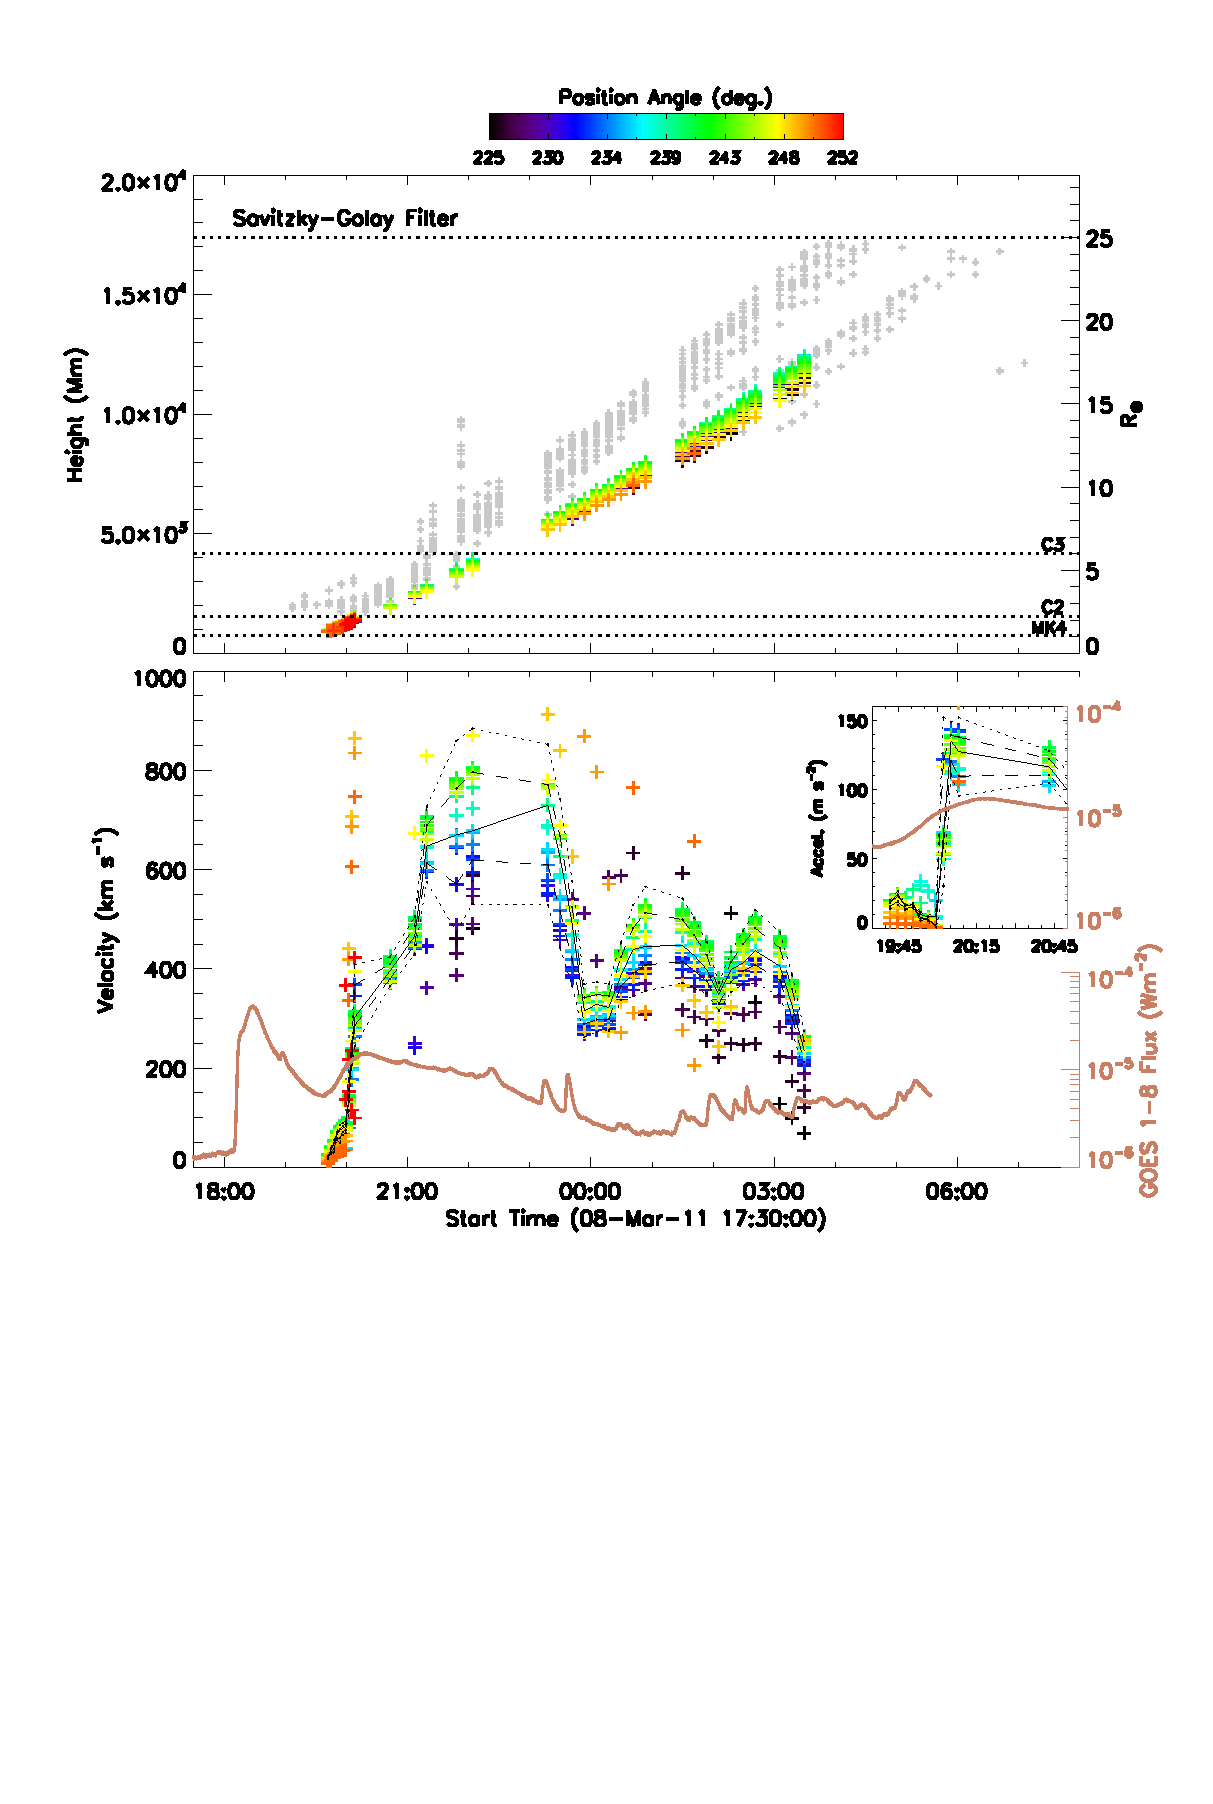
\includegraphics[clip=true, scale=0.63, trim=20 250 0 20]{images/plot_kins_quartiles_savgol_20110308T194136_goes.eps}}
\caption{The kinematic profiles of height, velocity, and (inset) the early acceleration phase of the CME core material, detected and characterized via the multiscale edge enhancement and ellipse-fits (see Section\,\ref{sect:techniques} and Figs.\,\ref{ell_heights_inner} and \ref{lasco_c2_fig}). The automated CORIMP CME detections provide the height-time measurements shown here in gray for reference, with the characterized CME core height-time measurements plotted in color according to their position angle. The fields-of-view of the MK4, C2 and C3 instruments are indicated by the horizontal dotted lines, covering a useable range of 1.1\,--\,25\,$R_{\odot}$, with the CME core tracked to approximately 18$\,R_{\odot}$. A Savitzky-Golar filter was applied to the height-time measurements to obtain distribution profiles of velocity and acceleration, with the median, interquartiles range, and upper/lower fences over-plotted in solid, dashed and dotted lines respectively. Overlaid is the GOES X-ray 1\,--\,8\,{\AA} flux profile, showing the double-eruption peaks at about 18:28 and 20:15\,UT, the latter of which underlies the CME jerk (jump in acceleration).}
\label{kins_CMEcore}
\end{figure}


\section{Discussion}
\label{sect:discussion}

The study of this particular event is of interest in the context of the flare-CME relationship. Firstly, the two-stage flaring profile of the erupting loop system is evidence for a secondary heating process, indicating two stages of magnetic reconnection that occur to first change the topology of the system and then allow for the subsequent flux rope eruption. This scenario demonstrates that a loss of stability occurs initially, to allow the loop system to rise and alter its magnetic configuration with an explosive energy release detected as an M-class flare. This is then followed by a secondary energy release that allows the underlying flux rope of the system to erupt through the corona as a CME, with the production of a second X-ray peak and post-flare loops at the CME footpoints.

It is not clear why we observe different rates of motion of the material in the SWAP and MK4 images during the CME onset (Fig.~\ref{ell_heights_inner}). The simplest reason is possibly that the material observed by the different instruments corresponds to different parts of the erupting structure that are difficult to dissociate from each other on the plane-of-sky. This could mean that line-of-sight effects are causing a discrepancy in the height-time profiles that appears as this offset in their rates of propagation. However, being a limb event, this seems too weak an argument for the large offset in the heights measured. While some cause for the offset may be attributed to a loss of signal in the EUV as the eruption proceeds, such an effect would not be strong enough to explain a consistently increasing offset of this magnitude since it would be expected that the white-light signal would undergo a similar effect in the MK4 observations. Indeed if the offset is true and the different parts of the structure (hotter EUV material versus cooler white-light material) do undergo different rates of propagation on the same plane-of-sky, it may be that the trailing part simply becomes a different portion of the main CME and/or undergoes a delayed jerk in its motion which is not observed as the EUV signal diminishes towards the edge of the SWAP field-of-view. This would imply that there is some form of delayed or staggered eruption occurring throughout the CME structure, or that expansion effects take over as the CME bubble forms, which act to create the observed offset between the different observations. 

%Alternatively, the different observations of the EUV and white-light may correspond to significantly different parts of the eruption undergoing different physical mechanisms as the system evolves, leading to their detection in the hotter EUV bands versus the cooler white-light images. The heating and cooling of loop structures over evolving active regions is well reported in observations, for example (refs?).

More intriguing is the possibility that this event is a good example of a breakout CME. The observations of \inlinecite{2013ApJS..206...19M} show a streamer swelling on the limb above the active region to large heights in the LASCO coronagraphs, that evolves slowly over the preceding days in the lead-up to the eruptive event; including being disturbed by an earlier CME that erupts to the northwest on March 7, and some faint brightenings and outward propagating blobs within the expanding helmet streamer loops indicative of interchange reconnection. Such activity has long been recognized as an observational precursor to CME initiation \cite{1993JGR....9813177H} though not always observed to such heights due to the low signal-to-noise ratio, overcome by the dynamic separation technique of \inlinecite{2012ApJ...752..144M}. For this active region it may be postulated that a form of external tether-cutting is occurring in the lead-up to, and most strongly at, the time of the main flare (M4.4; $\sim$18:08\,UT) that allows a change in the magnetic topology of the system such that the CME flux rope can form and then erupt at the time of the secondary flare (M1.4; $\sim$20:00\,UT). These observations suggest a form of breakout reconnection is driving the streamer blowout CME as modeled by \inlinecite{2009ApJ...693.1178V}, wherein they describe how the rising flux rope can ``snow plow" the plasma ahead of it. This has the effect of broadening the helmet streamer and facilitating breakout reconnection between the flux rope and the helmet field. Flare reconnection then sets in due to the expansion of the magnetic field in the wake of the erupting breakout arcade. These effects could account for the combined observations of this event; most notably the offset in the flux rope motion observed in EUV and the plasma motion observed in white-light, that form the core of the CME whose increased size may be attributed to the helmet streamer blowout. The measured jerk in the CME motion then coincides with the allowed blowout eruption through the breakout process while reconnection occurs behind, indicated by the elongated ``X"-shaped structure and post-flare loops in the AIA observations of \inlinecite{2012ApJ...746L...5S}.

\section{Conclusions}
\label{sect:conclusions}

The \emph{PROBA2}/SWAP imager is unique in that it provides extended EUV observations of the Sun and low-corona to greater heights than other EUV imagers such as \emph{SDO}/AIA. An ongoing goal in solar physics has been to study the connection between processes on the Sun and the effects felt elsewhere in the heliosphere; a connection known to lie predominantly within the regions of the photosphere, chromosphere and corona. Therefore obtaining and bridging observations across the solar atmosphere is paramount to understanding the physics at play. Since the LASCO/C1 coronagraph was lost very early on in the \emph{SOHO} mission, observations of the low corona have generally been quite limited. In order to bridge this gap and garner some knowledge of the low-corona initiation phase of CMEs, we have combined the SWAP observations with those of the ground-based MK4 coronagraph, to directly compare the EUV and white-light imagery. This was achieved through the use of advanced image processing techniques to overcome the low signal-to-noise ratio in these data, and characterize the erupting structures of interest. The subsequent investigation of the dynamics of a specific case-study on 8~March~2011 provides insight to the early CME formation and eruption. This compliments the previous investigation of \inlinecite{2012ApJ...746L...5S} who first reported on the event's two-stage flaring profile as evidence for secondary heating, but lacked the observational coverage of the CME's initiation phase as now determined with SWAP and MK4.

The combination of observations in this study, in association with the previous reported analyses of the event, provide a greater insight into the processes at play throughout the early phases of the eruption. The direct overlap of the SWAP and MK4 images, with methods in place to boost the signal-to-noise ratio of the structures of interest, nicely bridges the disk observations of AIA and the coronal observations of LASCO, allowing the eruption to be tracked across a range of heights not usually observed in this manner. The event chosen for study here highlights the importance of multi-wavelength, high-cadence, extensive coverage observations of the low-corona, where the physical mechanisms that underly CME formation, initiation, and connection with flares and surrounding coronal field may best be investigated. It is hoped that future instruments such as the new MLSO K-coronagraph\footnote{http://www.cosmo.ucar.edu/kcoronagraph.html} will help achieve this.


% \section{}%\label{s:?} 




%% Figure 
%
% \begin{figure} 
% \centerline{\includegraphics[width=0.5\textwidth,clip=]{<fig.eps>}}
% \caption{}%\label{fig:?}
% \end{figure}



%% Table
%
% \begin{table}
% \caption{}%\label{tbl:?}
% \begin{tabular}{}     
% \hline
% \multicolumn{2}{c}{<>}
% <data>
% \hline
% \end{tabular}
% \end{table}
  

%%%%%%%%%%%%%%%%%%%%%%%%%%%%%%%%%%%%%%%%%%%%%%%%%%%%%%%%%%%%%%%%%%%%%%%%%%%
%% Appendix
%
% \appendix   



%%%%%%%%%%%%%%%%%%%%%%%%%%%%%%%%%%%%%%%%%%%%%%%%%%%%%%%%%%%%%%%%%%%%%%%%%%%
%% Acknowledgements
%
 \begin{acks}
 
This work is supported by SHINE grant 0962716 and NASA grants NNX08AJ07G and NNX13AG11G to the Institute for Astronomy.
SWAP is a project of the Centre Spatial de Li'ege and the Royal Observatory of Belgium funded by the Belgian Federal Science Policy Office (BELSPO).
MK4 data is provided courtesy of the Mauna Loa Solar Observatory, operated by the High Altitude Observatory, as part of the National Center for Atmospheric Research (NCAR). NCAR is supported by the National Science Foundation.
The \emph{SOHO}/LASCO data used here are produced by a consortium of the Naval Research Laboratory (USA), Max-Planck-Institut fuer Aeronomie (Germany), Laboratoire d'Astronomie (France), and the University of Birmingham (UK). SOHO is a project of international cooperation between ESA and NASA.
\emph{SDO} data supplied courtesy of the NASA/\emph{SDO} consortia.

 \end{acks}


%%% %%%%%%%%%%%%%%%%%%%%%%%%%%%%%%%%%%%%%%%%%%%%%%%%%%%%%%%%%%%
%% Bibliography
%
% Using BibTeX
%
 \bibliographystyle{spr-mp-sola.bst}
% %\bibliographystyle{spr-mp-sola-cnd} %% Alternative style: no title, no concluding page
 \bibliography{references.bib}  
%
% Without BibTeX 
% \begin{thebibliography}{}
% \bibitem[\protect\citeauthoryear{Author}{Year}]{key}
%   <bibliographical entry>
%
% \bibitem[\protect\citeauthoryear{}{}]{}
%   
%  
% \end{thebibliography}

\end{article} 
\end{document}
